%%%%%%%%%%%%%%%%%%%%%%%%%%%%%%%%%%%%%%%%%%%%%%%%%%%%%%%%%%%%%%%%%%%%%%
%
%   Extreme motion generation, part II:
%   downstream-return seed selection over enumerated self-motion branches
%   Springer STAR series proceedings (svproc class)
%
%   Compile with:
%       pdflatex main
%       bibtex   main
%       pdflatex main
%       pdflatex main
%
%%%%%%%%%%%%%%%%%%%%%%%%%%%%%%%%%%%%%%%%%%%%%%%%%%%%%%%%%%%%%%%%%%%%%%

\documentclass{svproc}

% ---- Recommended packages (per Springer author instructions) ----
\usepackage{graphicx}
\usepackage[bottom]{footmisc}
\usepackage{multicol}
\usepackage{url}
\def\UrlFont{\rmfamily}

% ---- Self-defined packages
\usepackage{xcolor}
\usepackage{amsmath,amssymb}
\usepackage{booktabs}
\usepackage{threeparttable}
\usepackage{multirow}
\usepackage[hidelinks]{hyperref}
\usepackage{tikz}
\usetikzlibrary{arrows.meta,positioning,fit,calc}

\graphicspath{{figures/}}

% ---- Sealed final-holdout numbers: filled once after the single sealed read ----
\newcommand{\sealedNew}{0.5734}
\newcommand{\sealedOld}{0.5443}
\newcommand{\sealedDelta}{$+29.2$}
\newcommand{\sealedCI}{$[24.8,33.4]$}
\newcommand{\sealedTrim}{$+16.8$}
\newcommand{\sealedHarm}{38.3}
\newcommand{\sealedWin}{50.4}
\newcommand{\sealedCapture}{67.3}
\newcommand{\sealedOracle}{0.6336}

\begin{document}
\mainmatter

%%%%%%%%%%%%%%%%%%%%%%%%%%%%%%%%%%%%%%%%%%%%%%%%%%%%%%%%%%%%%%%%%%%%%%
\title{Where Extreme Motion Begins: Downstream-Return Seed Selection over
Enumerated Self-Motion Branches}
\titlerunning{Downstream-Return Seed Selection}

\author{Xinyi Yuan
        \and Weiwei Wan$^{*}$
        \and Kensuke Harada}
\authorrunning{Yuan et al.}
\tocauthor{Xinyi Yuan, Weiwei Wan, Kensuke Harada}

\institute{Graduate School of Engineering Science, The University of Osaka, Japan.}

\maketitle

%%%%%%%%%%%%%%%%%%%%%%%%%%%%%%%%%%%%%%%%%%%%%%%%%%%%%%%%%%%%%%%%%%%%%%
\begin{abstract}
In extreme motion generation, a fixed-base manipulator maximizes the Cartesian
path length along a pre-defined trajectory before any safety boundary is
violated. Prior work has shown that the achievable length is largely decided
before execution, by the choice of the initial joint configuration among the
disconnected branches of the self-motion manifold. This paper studies that
first decision as the opening macro-action of a two-stage semi-Markov decision
process and asks four questions: whether the candidate set itself bounds the
system, which supervision signal the selection requires, how much of the
long-horizon outcome is predictable from static information, and whether the
selection stage and the downstream controller must be adapted jointly. On
10{,}000-scale straight-line path-following tasks with a 7-DoF Franka FR3, we
find that (i)~replacing a learned generative proposal pool with direct
cone-constrained IK enumeration more than doubles the attainable headroom;
(ii)~on the enumerated pool every geometric surrogate fails, whereas a
selector supervised by complete closed-loop returns recovers about two thirds
of the headroom; (iii)~this fraction is a measured representability boundary:
granting the selector a full kinematic-lookahead oracle adds nothing;
(iv)~forward controller adaptation is verified to be unnecessary here, and a
novelty-stratified analysis explains why. The resulting system deploys as one
static selector forward, one seed, and one rollout, and lengthens the average
path by 24.5\,mm and 27.7\,mm over the strongest prior system on two held-out
sets of 2{,}048 tasks each; the gain is stable across six training seeds and
reaches $+29.2$\,mm on a sealed 10{,}000-task final holdout.
\keywords{extreme motion generation, seed selection, reinforcement learning}
\end{abstract}

%%%%%%%%%%%%%%%%%%%%%%%%%%%%%%%%%%%%%%%%%%%%%%%%%%%%%%%%%%%%%%%%%%%%%%
\section{Introduction}
\label{sec:intro}
Consider again a compact, fixed-base manipulator executing a coating or
welding operation along a straight line~\cite{yuan2026extreme}. The motion is
continuous and strictly constrained by safety boundaries such as joint limits
and tool-orientation tolerance, and in practice one of these boundaries is
violated long before the end-effector approaches the edge of the reachable
workspace. We refer to the problem of deferring these violations as
\textit{extreme motion generation}: maximizing the Cartesian path length along
a pre-defined trajectory within the manipulator's workspace.

Our previous study addressed the execution stage of this problem with a hybrid
controller and initialized the motion by sampling a conditional diffusion
model over favorable starting configurations~\cite{yuan2026extreme}. The
present paper turns to the initialization stage itself, motivated by a
structural fact of redundant manipulation. For a task that constrains fewer
degrees of freedom than the arm possesses, the feasible initial configurations
form a self-motion manifold whose joint-limit-induced branches are
disconnected; configurations on different branches realize the same
end-effector pose yet differ sharply in how far the subsequent motion can
proceed. Three properties make this initial choice scientifically distinctive.
First, it is \textit{decisive}: on our task distribution, the best and worst
feasible starting configurations of the same task differ by a median of
472\,mm of final path length, more than 85\,\% of the average task length.
Second, its consequence is \textit{revealed late}: whether a branch survives
is dominated by orientation-cone violations that occur deep into the
trajectory, and, as we show, is only weakly visible in any instantaneous
geometric quantity at $t{=}0$. Third, the decision must be made
\textit{without trial}: an execution budget of one rollout per task excludes
probing candidates, and because a full episode lasts only about 55 control
steps, any informative probe would cost nearly as much as exhaustive
execution. The initial choice must therefore compress the outcome of an entire
closed-loop execution into a single static decision.

We formalize the initial configuration as the first, discrete macro-action of
a two-stage semi-Markov decision process whose continuation is the continuous
low-level controller, and whose shared objective is the final path length.
This formulation admits two coupling directions in the sense of sequential
policy chaining~\cite{chen2023sequential}: a \textit{backward} direction, in
which complete controller returns supervise the selection, and a
\textit{forward} direction, in which the controller adapts to the
selection-induced initial-state distribution. Rather than assuming both
directions are necessary, we treat their necessity as an experimental
question. The contributions are four measured answers:

\begin{enumerate}
\item \textbf{The candidate set bounds the system.} Replacing the learned
generative proposal pool of~\cite{yuan2026extreme} with direct
cone-constrained IK enumeration and farthest-point selection raises the
per-task attainable ceiling by 52\,mm on average and more than doubles the
selectable headroom; the ceiling saturates by pool size $K{\approx}16$--$24$,
so enumeration coverage, not a learned generator, is what matters
(Sec.~\ref{sec:pool}).
\item \textbf{Backward credit is necessary, not auxiliary.} On the enumerated
pool, every static geometric surrogate and every selector transferred from the
generative pool performs \textit{worse} than a trivial first-feasible rule,
while the same feature set supervised by complete closed-loop returns recovers
62--68\,\% of the oracle headroom (Sec.~\ref{sec:backward}).
\item \textbf{The static limit is measured, not conjectured.} Capture
plateaus near two thirds under capacity, schedule, and architecture variation,
and---decisively---granting the selector an exact kinematic-lookahead feature,
computed by integrating the damped tracking field to termination, leaves
capture unchanged. The residual third of the headroom requires information
about the learned controller's own closed-loop behavior, which no static
quantity can carry (Sec.~\ref{sec:boundary}).
\item \textbf{Forward adaptation is verified unnecessary here.} Two
progressively better-engineered rounds of controller adaptation on the
selection-induced distribution yield a null effect, the loop's fail-closed
gate rejecting one harmful and one neutral update. A novelty-stratified
analysis shows the adaptation gain is zero even for seeds 3--8\,rad away from
any configuration the prior pool contained, and explains the mechanism:
task-relative observations combined with training over $10^{5}$ random tasks
already cover the relative state space that new branches occupy
(Sec.~\ref{sec:coupling}).
\end{enumerate}

The deployed system keeps the strictest execution budget---one selector
forward, one seed, one controller rollout, no probes---and lengthens the
average path by 24.5\,mm and 27.7\,mm over the strongest prior system on two
held-out sets of 2{,}048 tasks (95\,\% CIs $[16.1,33.0]$ and $[18.5,36.9]$),
with a 5\,\% trimmed gain of 14.6\,mm and 18.0\,mm confirming that typical
tasks, not only tail cases, improve. The result is stable across six selector
training seeds and reaches $+29.2$\,mm (CI $[24.8,33.4]$) on a sealed
10{,}000-task holdout generated after every design decision was frozen.

%%%%%%%%%%%%%%%%%%%%%%%%%%%%%%%%%%%%%%%%%%%%%%%%%%%%%%%%%%%%%%%%%%%%%%
\section{Related Work}

\subsection{Initialization of Redundant Manipulation}
The influence of the initial configuration on downstream feasibility has long
been recognized in redundancy resolution. Classical treatments optimize
instantaneous criteria such as manipulability~\cite{yoshikawa1985manipulability}
or joint-limit distance, and modern planners embed these measures into
sampling and cost~\cite{shen2023adaptive,cai2025just}. Generative approaches
model the full inverse-kinematics solution set, either with normalizing
flows~\cite{ames2022ikflow} or diffusion models~\cite{zhang2025ikdiffuser},
and DiffusionSeeder~\cite{huang2024diffusionseeder} seeds downstream motion
with multi-modal trajectory initializations, closely related to the
conditional sampler of our prior system~\cite{yuan2026extreme}. All of these
methods score or generate initializations from information available at
$t{=}0$. Our experiments quantify exactly how far such information can go on a
long-horizon objective: instantaneous surrogates fail outright on a diverse
candidate set, learned static selection recovers two thirds of the headroom,
and the remainder is shown to be invisible to any static feature, including an
exact kinematic continuation.

\subsection{Chaining and Bidirectional Policy Adaptation}
Sequential Dexterity~\cite{chen2023sequential} fine-tunes adjacent sub-policies
bidirectionally through a transition-feasibility function so that each skill
terminates inside the basin of its successor. Our two-stage decomposition
borrows this credit structure---the first stage must be evaluated by the
success of the second---but differs in what the experiments support. In our
system the backward direction carries the entire gain, while the forward
direction is verified to be already saturated by the controller's design; we
provide a falsifiable coverage-based explanation and delineate when forward
adaptation should become necessary. We view this as complementary evidence:
the value of each chaining direction is a property of the system, to be
measured rather than assumed.

\subsection{Learning from Complete Returns}
Supervising a fast decision-maker with the outcome of an expensive full
evaluation follows the pattern of expert iteration and amortized
planning~\cite{yuan2026iksel}. Here the expensive evaluation is the complete
closed-loop rollout of every feasible candidate under a frozen controller, and
the amortized decision is a listwise selector queried once per task. Unlike
distillation from a search teacher, the complete return table is exhaustive
over the discrete action set, so the selector's residual error isolates the
representability of the outcome, a property we exploit in
Sec.~\ref{sec:boundary}.

%%%%%%%%%%%%%%%%%%%%%%%%%%%%%%%%%%%%%%%%%%%%%%%%%%%%%%%%%%%%%%%%%%%%%%
\section{Problem Formulation}
\label{sec:formulation}
We adopt the task setting of~\cite{yuan2026extreme}. A straight-line
path-following task is specified by the condition vector
$\mathbf{c} = [\mathbf{p}_{0}, \mathbf{d}, \mathbf{n}] \in \mathbb{R}^{9}$,
where $\mathbf{p}_{0}$ is the starting position and $\mathbf{d}$, $\mathbf{n}$
are unit vectors giving the motion direction and the task-plane normal. A
7-DoF manipulator with configuration $\mathbf{q}\in\mathbb{R}^{7}$ must keep
its end-effector position $\mathbf{p}(\mathbf{q})$ within
$\epsilon_{\text{pos}}$ of the advancing reference on the line and its tool
axis $\mathbf{z}(\mathbf{q})$ within a cone of half-angle $\theta_{\max}$
about $\mathbf{n}$, subject to joint limits; the episode terminates at the
first violation, and the objective $\mathcal{L}$ is the net path length
achieved before termination.

The two decisions of the system are made at different time scales, which we
capture as a two-stage semi-Markov decision process. At $t{=}0$, a discrete
macro-action selects the initial configuration from a finite feasible set
$Q(\mathbf{c})=\{\mathbf{q}_{1},\dots,\mathbf{q}_{K}\}$ produced by a
candidate generator; for $t{>}0$, the continuous controller
$\pi_{\mathrm{ctrl}}$ acts at every step. Both stages share the terminal
objective:
\begin{equation}
\label{eq:smdp}
\max_{\phi,\theta}\;
\mathbb{E}_{\mathbf{c}}\!\left[
\mathcal{L}\big(\mathbf{q}_{i},\,\pi_{\mathrm{ctrl},\theta};\,\mathbf{c}\big)
\right],
\qquad i \sim \pi_{\mathrm{seed},\phi}(\,\cdot\mid \mathbf{c}, Q(\mathbf{c})).
\end{equation}
Deployment is restricted to \textit{one static pass}: the selector network is
evaluated once, commits to a single $\mathbf{q}_{0}$, and the controller
executes exactly one episode. No candidate probing, model-based rollout, or
replanning is permitted at execution time. This restriction is not incidental:
because episodes average only 55 steps, a probe long enough to reveal a
branch's fate costs nearly a full episode per candidate, collapsing any
probing scheme into exhaustive execution. The scientific content of the
problem is therefore whether, and to what extent, the terminal outcome of
Eq.~\eqref{eq:smdp} can be predicted from information available before motion
begins.

%%%%%%%%%%%%%%%%%%%%%%%%%%%%%%%%%%%%%%%%%%%%%%%%%%%%%%%%%%%%%%%%%%%%%%
\section{Method}
\label{sec:method}
Figure~\ref{fig:system} summarizes the system. We describe the three
components in the order they answer the questions of
Sec.~\ref{sec:intro}.

\begin{figure}[!tbp]
\centering
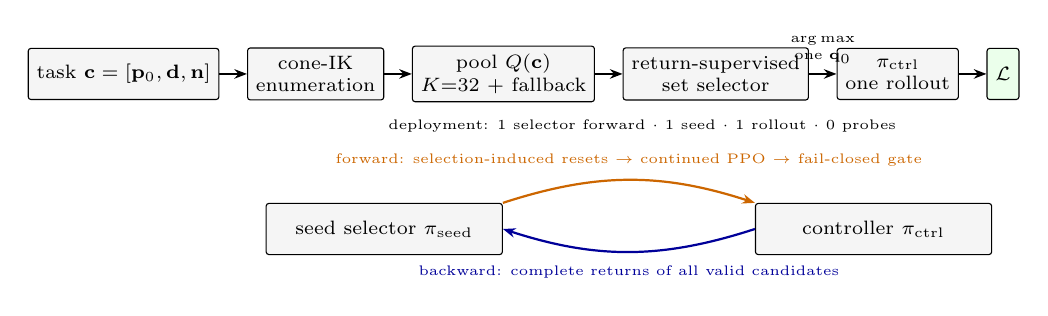
\begin{tikzpicture}[
  font=\scriptsize,
  box/.style={draw, rounded corners=1pt, fill=black!4, inner sep=3pt,
              minimum height=6.5mm, align=center},
  gbox/.style={box, fill=green!8},
  arr/.style={-{Stealth[length=1.6mm]}, thick},
  barr/.style={arr, blue!60!black},
  oarr/.style={arr, orange!80!black},
  lbl/.style={font=\tiny, align=center}]
% ---- deployment row ----
\node[box] (task) {task $\mathbf{c}=[\mathbf{p}_0,\mathbf{d},\mathbf{n}]$};
\node[box, right=3.5mm of task] (ik) {cone-IK\\enumeration};
\node[box, right=3.5mm of ik] (pool) {pool $Q(\mathbf{c})$\\$K{=}32$ + fallback};
\node[box, right=3.5mm of pool] (sel) {return-supervised\\set selector};
\node[box, right=3.5mm of sel] (ctrl) {$\pi_{\mathrm{ctrl}}$\\one rollout};
\node[gbox, right=3.5mm of ctrl] (L) {$\mathcal{L}$};
\draw[arr] (task) -- (ik);
\draw[arr] (ik) -- (pool);
\draw[arr] (pool) -- (sel);
\draw[arr] (sel) -- node[above, lbl] {$\arg\max$\\one $\mathbf{q}_0$} (ctrl);
\draw[arr] (ctrl) -- (L);
\node[lbl, below=1mm of pool.south east, anchor=north, xshift=6mm]
  {deployment: 1 selector forward $\cdot$ 1 seed $\cdot$ 1 rollout $\cdot$ 0 probes};
% ---- training loop ----
\node[box, below=13mm of ik.south east, minimum width=30mm] (seed)
  {seed selector $\pi_{\mathrm{seed}}$};
\node[box, right=32mm of seed, minimum width=30mm] (c0)
  {controller $\pi_{\mathrm{ctrl}}$};
\draw[barr] (c0.west) to[bend left=18]
  node[below, lbl, yshift=-0.5mm]
  {\textcolor{blue!60!black}{backward: complete returns of all valid candidates}}
  (seed.east);
\draw[oarr] (seed.north east) to[bend left=18]
  node[above, lbl, yshift=0.5mm]
  {\textcolor{orange!80!black}{forward: selection-induced resets
   $\rightarrow$ continued PPO $\rightarrow$ fail-closed gate}}
  (c0.north west);
\end{tikzpicture}
\caption{The two-stage system. Top: the deployed path is one static selector
forward over an enumerated cone-IK pool, followed by a single controller
rollout. Bottom: the training loop transports terminal credit backward through
complete candidate rollouts, and attempts forward controller adaptation on the
selection-induced reset distribution behind a fail-closed promotion gate;
on this task, the gate retains the original controller
(Sec.~\ref{sec:coupling}).}
\label{fig:system}
\end{figure}

\subsection{Enumerated Candidate Pool}
\label{sec:method-pool}
Instead of sampling a learned generative model, the candidate layer
enumerates the feasible set directly. For each task, 128 damped-least-squares
IK problems are solved from mixed random restarts toward tool directions
sampled within the orientation cone, followed by joint-space deduplication at
0.08\,rad; the median task yields 48 distinct solutions spread over the
disconnected self-motion branches. Farthest-point selection in joint space
then retains $K{=}32$ candidates, and the classical fallback configuration
of~\cite{yuan2026extreme} is appended as a designated final slot. Every
candidate passes strict physical validation---joint limits, 5\,mm position
error, the $\theta_{\max}$ cone, and collision---before entering the action
set; 94\,\% of slots are valid on average. Diversity, not count, is the
operative property: the attainable ceiling saturates by $K{\approx}16$--$24$
under farthest-point ordering (Sec.~\ref{sec:pool}), and enumeration density
rather than a learned prior determines coverage.

\subsection{Backward Credit: Return-Supervised Selection}
\label{sec:method-selector}
With the controller frozen, every valid candidate of every training task is
rolled out to termination, producing a complete per-candidate return table.
The selector is a five-member ensemble; each member embeds the $K$
candidates' 45-dimensional features---the controller's initial observation
augmented with the ray error, log positional manipulability, and ten
task-aligned differential-kinematics descriptors~\cite{yuan2026extreme}---with
a permutation-equivariant encoder whose mean-pooled context is concatenated
back to each candidate. Two heads are trained jointly: a listwise scoring
head fit to within-task range-normalized returns by softmax cross-entropy,
and a feasibility head regressing the return in metres under a Huber loss.
Members are trained on task-level bootstrap resamples and aggregated by mean
score; deployment is the masked $\arg\max$ over valid candidates. The
complete table, rather than sampled actions, is what makes the supervision a
property of the \textit{problem}: any residual selection error measures what
the features cannot express, not what the data failed to visit.

\subsection{Forward Adaptation under a Fail-Closed Gate}
\label{sec:method-forward}
The forward direction freezes the selector and continues PPO training of the
controller on the reset distribution it induces, mixing 70\,\% selector
samples with 20\,\% uniform-valid and 10\,\% fallback resets to prevent
collapse. Candidate controllers are admitted only through a promotion gate
evaluated on paired held-out statistics; a rejected candidate leaves the
deployed controller untouched. As Sec.~\ref{sec:coupling} reports, both
attempted rounds were declined---one as harmful, one as neutral---so the
deployed system retains the original controller, and the gate's audit trail
becomes part of the scientific result.

%%%%%%%%%%%%%%%%%%%%%%%%%%%%%%%%%%%%%%%%%%%%%%%%%%%%%%%%%%%%%%%%%%%%%%
\section{Experimental Setup}
\label{sec:setup}
All experiments use the straight-line path-following distribution
of~\cite{yuan2026extreme} with a simulated 7-DoF Franka FR3: tasks are drawn
from a pool of $10^{5}$ random lines, and the controller is the pure RL
policy trained in that system. The prior system---the conditional diffusion
proposal pool with its learned five-member ranker, deployed on the same
controller---serves as the baseline throughout; we reuse its cached
per-candidate rollouts so that both systems are compared on identical tasks
under an identical controller.

Training uses 18{,}432 tasks with complete candidate rollouts
($5.7\times10^{5}$ episodes). Model development decisions are made
exclusively on a geometry-disjoint internal split (exact float32 task
signatures; 3{,}000 held-out tasks); the two evaluation sets---the 2{,}048-task
validation split and a 2{,}048-task external set built from a fresh line
pool with audited zero geometry overlap---are read only for the results
reported here. A sealed 10{,}000-task holdout was generated from fresh pool,
task, and enumeration seeds after all rules, weights, and the selector
publication rule (median across training seeds) were frozen and
preregistered; it is read once, by the published selector only. We report
paired per-task statistics against the baseline: the mean difference with a
20{,}000-resample bootstrap 95\,\% CI, the 5\,\% two-sided trimmed mean, and
the fraction of tasks changed by more than $\pm1$\,mm, alongside the fraction
of the pool's oracle headroom captured,
$(\mathcal{L}_{\mathrm{sel}}-\mathcal{L}_{\mathrm{first}})/
 (\mathcal{L}_{\mathrm{oracle}}-\mathcal{L}_{\mathrm{first}})$.

%%%%%%%%%%%%%%%%%%%%%%%%%%%%%%%%%%%%%%%%%%%%%%%%%%%%%%%%%%%%%%%%%%%%%%
\section{Results}
\label{sec:results}

\subsection{The Candidate Pool Bounds the System}
\label{sec:pool}
Table~\ref{tab:pool} and Fig.~\ref{fig:pool} compare the enumerated pool with
the generative proposal pool on the 18{,}432 training tasks under the frozen
controller. Enumeration raises the mean per-task ceiling from 0.582\,m to
0.634\,m ($+52.1$\,mm; a better best exists on 68.4\,\% of tasks against
16.8\,\% for the converse) and widens the selectable headroom from 84.5\,mm to
180.6\,mm per task. The within-task spread between the best and worst feasible
candidate (Fig.~\ref{fig:spread}) shifts from a median of 145\,mm to 472\,mm:
where the generative pool proposes near-duplicates of one good region, the
enumerated pool spans branches whose outcomes differ by the scale of the task
itself. The oracle curve saturates by $K{\approx}16$--$24$ under
farthest-point ordering (98.4\,\% of the $K{=}32$ ceiling at $K{=}16$), so the
benefit is branch coverage rather than candidate count. On the small fraction
of tasks whose enumerated pool still lacks a competitor to the baseline's
choice (6--8\,\% of dev tasks), tripling the enumeration budget closes
71--73\,\% of the remaining gap and turns its mean sign negative, confirming
an enumeration-coverage artifact rather than a manifold limitation; a learned
generator is not required at any point.

\begin{table}[!tbp]
\centering
\caption{Candidate pools under the identical frozen controller
(18{,}432 training tasks). Oracle = best valid candidate per task.}
\label{tab:pool}
\begin{tabular}{lcc}
\toprule
 & generative pool ($K{=}8{+}1$) & enumerated pool ($K{=}32{+}1$) \\
\midrule
valid candidates / task & 7.9 & 31.0 \\
first-feasible [m] & 0.494 & 0.453 \\
oracle [m] & 0.582 & \textbf{0.634} \\
headroom (oracle $-$ first) [mm] & 84.5 & \textbf{180.6} \\
within-task spread, median [mm] & 145 & \textbf{472} \\
\bottomrule
\end{tabular}
\end{table}

\begin{figure}[!tbp]
\centering
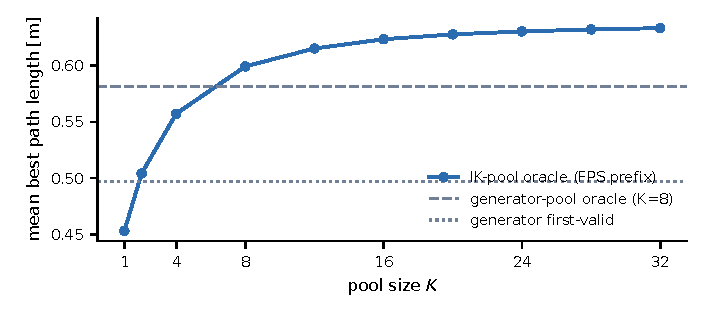
\includegraphics[width=\linewidth]{fig_oracle_vs_k.pdf}
\caption{Attainable ceiling versus pool size. The enumerated-pool oracle
(farthest-point prefix) passes the full generative-pool oracle by $K{=}4$ and
saturates by $K{\approx}16$--$24$; marginal value at the tail is
0.2\,mm per four candidates.}
\label{fig:pool}
\end{figure}

\begin{figure}[!tbp]
\centering
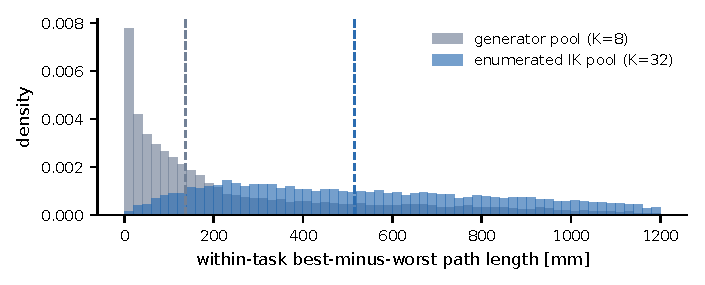
\includegraphics[width=\linewidth]{fig_spread.pdf}
\caption{Within-task best-minus-worst final path length. The enumerated pool
(median 472\,mm) exposes outcome diversity that the generative pool
(median 145\,mm) compresses away.}
\label{fig:spread}
\end{figure}

\subsection{Backward Credit is Necessary}
\label{sec:backward}
Table~\ref{tab:necessity} isolates the supervision signal on the enumerated
pool. Every selection rule built from instantaneous information fails: the
selector ensemble of the prior system, transferred unchanged, captures
$-25$\,\% of the headroom (worse than taking the first feasible candidate),
and the strongest single geometric feature---a component of the damped
line-tracking joint velocity, with a within-task rank correlation of only
0.28---captures $-23$\,\%. The identical 45-dimensional feature set, retrained
with complete closed-loop returns as targets, captures 62.7\,\% at 15{,}000
training tasks (66.6\,\% for the member ensemble), with a per-seed standard
deviation of 0.2 percentage points. Figure~\ref{fig:scaling} traces the
supervision from 1{,}000 tasks upward; even a plain ridge regression on the
same features reaches 23.6\,\%, confirming that the signal enters through the
labels, not the model class. On this pool, downstream-return supervision is
the difference between failing and working, which elevates backward credit
transport from a refinement to a requirement.

\begin{table}[!tbp]
\centering
\caption{Selection rules on the identical enumerated pool
(held-out tasks; capture of oracle headroom).}
\label{tab:necessity}
\begin{tabular}{llr}
\toprule
selection rule & supervision & capture [\%] \\
\midrule
first feasible & none & 0.0 \\
best single geometric feature & none & $-23.1$ \\
prior-system selector, transferred & generative-pool returns & $-25.8$ \\
ridge on 45-D features & complete returns & $+23.6$ \\
listwise selector (single) & complete returns & $+62.7\pm0.2$ \\
listwise selector (ensemble) & complete returns & $\mathbf{+66.6}$ \\
\bottomrule
\end{tabular}
\end{table}

\begin{figure}[!tbp]
\centering
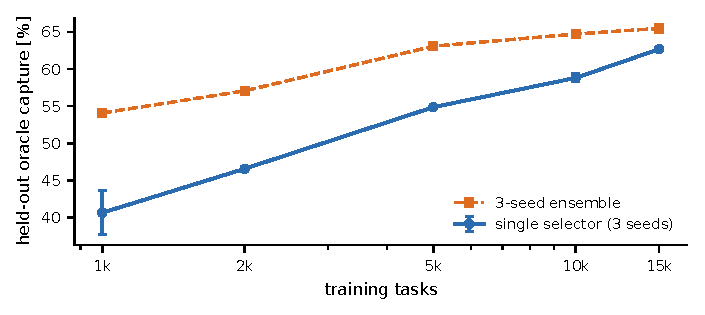
\includegraphics[width=\linewidth]{fig_scaling.pdf}
\caption{Held-out capture versus training-set size (geometry-disjoint
internal split). Seed-level scatter collapses as data grows; capacity and
schedule variations at the right end change nothing
(Sec.~\ref{sec:boundary}).}
\label{fig:scaling}
\end{figure}

\subsection{The Static Representability Boundary}
\label{sec:boundary}
Two thirds of the headroom is also where static prediction stops. Widening
the network, doubling its depth of training, and exchanging the encoder all
leave held-out capture at the same plateau
(58.6--61.9\,\% single, 62.9--66.6\,\% ensemble). The decisive experiment
grants the selector the strongest static information that exists: for every
candidate we integrate the damped line-tracking field on the pure kinematic
model until a constraint is met---a full nonlinear continuation of the
starting branch, requiring no environment step and no policy call. This
\textit{kinematic lookahead} is individually excellent: its within-task rank
correlation with the true outcome is 0.55, matching the entire trained
network (0.53), and its $\arg\max$ alone captures 52\,\% of the headroom. Yet
appended to the 45 features and retrained, it moves capture by nothing
($62.3\pm0.9$ single, 66.5 ensemble): the network had already internalized
the kinematic continuation from its one-step descriptors. The plateau is
therefore a measured boundary, not an engineering shortfall. What the
boundary excludes is identified by the lookahead itself: the kinematic field
survives 0.27\,m on average where the learned controller achieves 0.415\,m,
and this behavioral surplus---how the policy spends the null space that no
fixed field anticipates---is precisely the component of the outcome that
static selection cannot see and that only execution reveals.

\subsection{Forward Adaptation is Already Saturated}
\label{sec:coupling}
The forward direction was attempted twice under the promotion gate. A naive
continuation of PPO on the selection-induced resets degraded the external set
significantly ($-2.75$\,mm, CI $[-4.7,-1.1]$) and was rejected. A
properly-engineered second round---critic-only warm-up, zero entropy bonus, a
tightened KL trust region, and a fourfold budget---was harmless but null
(validation $+2.2$, CI $[-0.1,+4.6]$; external $-1.5$, CI $[-4.0,+1.0]$), with
the training reward saturated at 0.99 throughout: under its own objective the
controller had nothing left to learn from these states. Completing the loop
regardless---relabeling all $5.7\times10^{5}$ candidate rollouts under the
adapted controller and retraining the selector---left every cell of the
resulting $2{\times}2$ decomposition statistically tied, so the loop converges
to its first iterate.

Figure~\ref{fig:novelty} explains why, and makes the explanation falsifiable.
Stratifying tasks by the joint-space distance between the newly selected seed
and the nearest configuration available to the prior pool, the selector is
seen to move far across the manifold: the median chosen seed lies 2.16\,rad
(90th percentile 4.61\,rad) from anything the generative pool offered. If the
controller harbored a coverage gap, adaptation gains would concentrate in the
most novel stratum; instead the forward effect is zero in every quartile
(top quartile $+0.09\pm5.2$\,mm), and the unadapted controller performs
\textit{best} from the most novel branches (0.599\,m versus 0.528\,m in the
least novel quartile). The mechanism is the product of three design choices
inherited from~\cite{yuan2026extreme}: task-relative observations, training
over $10^{5}$ random tasks, and reset mixtures containing uniform feasible
configurations. In the relative state space the policy actually observes, an
unfamiliar branch of one task is a familiar state of another, so the
distribution shift that forward adaptation would repair has been absorbed in
advance. Conversely, this delineates where the forward direction should
matter: small task pools, absolute observations, or transfer to physical
hardware.

\begin{figure}[!tbp]
\centering
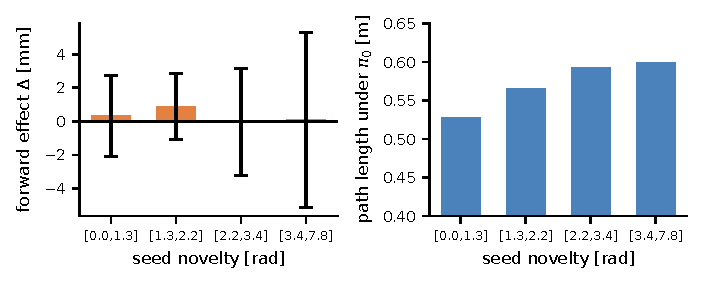
\includegraphics[width=\linewidth]{fig_novelty.pdf}
\caption{Novelty-stratified test of forward adaptation (both dev sets,
4{,}096 tasks). Left: adaptation effect by quartile of joint-space distance
from the selected seed to the nearest prior-pool configuration; all
quartiles are null. Right: the \textit{unadapted} controller's path length
rises with novelty---the selector seeks distant branches because they are
better, and the controller already exploits them.}
\label{fig:novelty}
\end{figure}

\subsection{System Comparison}
\label{sec:main}
Table~\ref{tab:main} reports the deployed system---enumerated pool, published
return-supervised selector, original controller, one static pass---against
the prior system on identical tasks. The mean path lengthens by 24.5\,mm
(validation) and 27.7\,mm (external), roughly fifteen times the margin the
prior system's own selector iteration achieved over its geometric
predecessor, and the 5\,\% trimmed means of $+14.6$ and $+18.0$\,mm show the
gain is carried by typical tasks rather than a heavy tail.
Figure~\ref{fig:delta} displays the full paired distribution: 51\,\% of tasks
improve by more than 1\,mm while 38\,\% regress---the enumerated pool's weak
first-feasible anchor means selection errors are costlier than in the
generative pool, and a risk-sensitive selection objective is the natural next
lever. Across six independent selector training seeds the gain is
$25.5\pm1.7$\,mm (validation) and $26.9\pm1.5$\,mm (external)%
\footnote{Run seeds $\{0,41000,\dots,45000\}$ under the preregistered
protocol; the frozen median rule published run~0, which is also the deployed
selector.}, and on the
sealed 10{,}000-task holdout, read once with the published selector, the gain
is \sealedDelta\,mm (CI \sealedCI, trimmed \sealedTrim\,mm, capture
\sealedCapture\,\%). Deployment cost is unchanged where it matters: the
selector forward remains sub-millisecond per task batched, candidate
enumeration adds roughly half a second of offline kinematics per task, and
the single controller rollout continues to dominate end-to-end latency.

\begin{table}[!tbp]
\centering
\begin{threeparttable}
\caption{Deployed system versus the prior system (identical tasks and
controller; paired statistics; positive favors ours).}
\label{tab:main}
\begin{tabular}{lccc}
\toprule
 & validation (2{,}048) & external (2{,}048) & sealed (10{,}000) \\
\midrule
prior system [m] & 0.5384 & 0.5518 & \sealedOld \\
ours [m] & \textbf{0.5629} & \textbf{0.5795} & \textbf{\sealedNew} \\
$\Delta$ mean [mm] & $+24.5$ & $+27.7$ & \sealedDelta \\
95\,\% CI [mm] & $[16.1,33.0]$ & $[18.5,36.9]$ & \sealedCI \\
$\Delta$ trimmed 5\,\% [mm] & $+14.6$ & $+18.0$ & \sealedTrim \\
win / harm $>$1\,mm [\%] & 51.8 / 37.0 & 50.4 / 39.0 & \sealedWin\,/\,\sealedHarm \\
oracle capture [\%] & 67.2 & 68.9 & \sealedCapture \\
\bottomrule
\end{tabular}
\begin{tablenotes}\footnotesize
\item Capture is measured against each pool's own complete-candidate oracle;
the enumerated pool's oracle is itself 52\,mm higher (Table~\ref{tab:pool}).
\end{tablenotes}
\end{threeparttable}
\end{table}

\begin{figure}[!tbp]
\centering
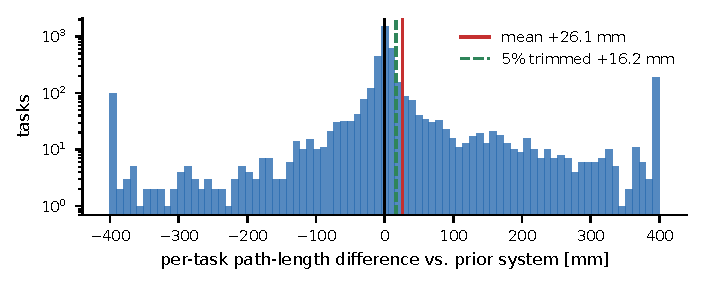
\includegraphics[width=\linewidth]{fig_delta_hist.pdf}
\caption{Per-task paired differences against the prior system (both dev
sets; log-scaled counts; clipped at $\pm400$\,mm for display). The trimmed
mean remains strongly positive: the improvement is not a tail artifact.}
\label{fig:delta}
\end{figure}

\subsection{Audit of the Bidirectional Loop}
\label{sec:audit}
Because every update passed through preregistered gates, the loop leaves a
complete decision trail: the first backward round was promoted
($+24.5/+27.7$\,mm); forward round one was rejected as harmful; forward round
two was declined as null; the second backward round, trained on relabeled
returns, tied its predecessor ($-0.3$\,mm) and was not promoted; capacity,
schedule, and lookahead-feature extensions were each declined on the internal
split. Two further negative results complete the record. A margin gate that
falls back to the classical seed raised harm instead of lowering it (37\,\%
$\rightarrow$ 50\,\%), because the enumerated pool's fallback is itself weak;
safe abstention requires a strong anchor, which this pool intentionally does
not contain. And the loop's convergence to its first iterate is not a failure
of the framework but its verdict: on this system, the coupling between
initialization and control lives entirely in the initialization.

%%%%%%%%%%%%%%%%%%%%%%%%%%%%%%%%%%%%%%%%%%%%%%%%%%%%%%%%%%%%%%%%%%%%%%
\section{Limitations}
\label{sec:limitations}
The remaining third of the headroom is shown to require execution-time
information, and we do not offer a static route to it; whether an extremely
short learned probe could price that information below oracle cost is open.
Thirty-eight percent of tasks regress relative to the prior system despite
the strongly positive mean and trimmed mean; a risk-sensitive selection
objective is unexplored. All findings are in simulation under a single task
family, and the coverage argument of Sec.~\ref{sec:coupling} predicts---but
does not verify---that forward adaptation becomes necessary on physical
hardware.

\section{Conclusion}
\label{sec:conclusion}
We studied the opening decision of extreme motion generation as the first
macro-action of a two-stage SMDP and measured, rather than assumed, each
property of the problem: the candidate set was the binding constraint until
enumeration replaced generation; complete downstream returns are the only
supervision under which static selection works at all; static prediction
ends, measurably, at two thirds of the headroom; and the forward coupling
direction is already saturated by the controller's design. The deployed
system converts these answers into a 24--28\,mm average extension of the
achievable path at an unchanged execution budget of one seed and one rollout,
confirmed across training seeds and a sealed holdout. We believe the same
measurement discipline---treating each direction of a modular pipeline's
coupling as a hypothesis with a preregistered gate---transfers beyond this
task.

%%%%%%%%%%%%%%%%%%%%%%%%%%%%%%%%%%%%%%%%%%%%%%%%%%%%%%%%%%%%%%%%%%%%%%
\bibliographystyle{unsrt}
\bibliography{references}

\end{document}
